\documentclass{standalone}
\usepackage{amssymb}
\usepackage{tikz}
\usetikzlibrary{
  arrows,
  automata,
  fit,
  positioning
}
\tikzset{
  ->,
  >=stealth,
  node distance = 0.5cm and 1cm,
  every state/.style = {thick},
  initial text = $ $,
}

\begin{document}
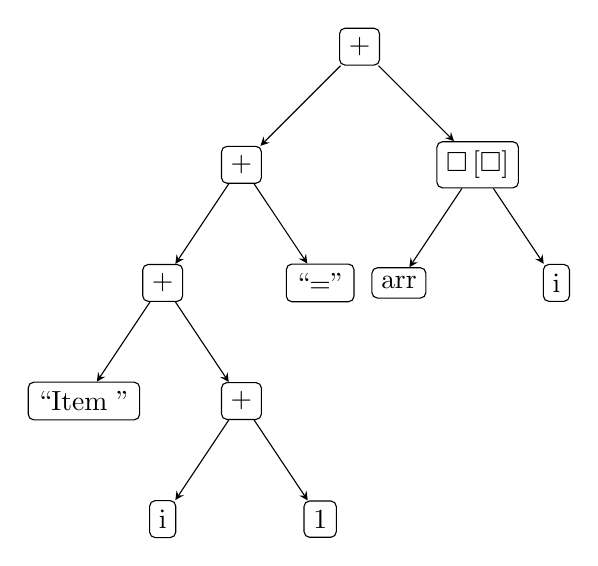
\begin{tikzpicture}[level 1/.style={sibling distance=3cm},
                    level 2/.style={sibling distance=2cm}]
\tikzstyle{every node}+=[draw, rectangle, rounded corners=2pt]
\node (a)[node distance=8cm] {$ + $}
      child { node { $ + $ } 
            child { node {$ + $ }
                    child { node { ``Item '' } }
                    child { node { $ + $ }
                            child { node { i } }
                            child { node { $ 1 $ } }
                    }
            }
            child { node { ``='' } }
      }
      child { node {$ \square \left[ \square \right] $} 
            child { node { arr } }
            child { node { i } }
      }
      ;
\end{tikzpicture}
\end{document}
